%%%%%%%%%%%%%%%%%%%%%%%%%%%%%%%%%%%%%%%%%%%%%%%%%%%%%%%%%%
%  Copyright (C) 2005 WanT group                         %
%  This file is distributed under the terms of the       %
%  GNU General Public License.                           %
%  See the file `License'  in the root directory of      %
%  the present distribution,                             %
%  or http://www.gnu.org/copyleft/gpl.txt                %
%%%%%%%%%%%%%%%%%%%%%%%%%%%%%%%%%%%%%%%%%%%%%%%%%%%%%%%%%%

\thispagestyle{empty}
\section{How to run \WANT\ : a step by step description}\label{section:run}

\noindent \underline {NOTE}: At present the \WANT\ code is
implemented to work as post processing of the self-consistent
calculations done using the Pwscf package (www.pwscf.org); thus we
will refer to that code in the following description.\\

\noindent Following the theoretical description of
Section~\ref{section:intro}, the evaluation of transport
properties requires a three separate steps:

\begin{enumerate}
\item Calculation of DFT-PW electronic structure:
\item Calculation of maximally-localized Wannier functions
\item Calculation of the quantum conductance
\end{enumerate}

\noindent \underline{IMPORTANT}: For a correct results, the
following steps $***$MUST$***$ be done in this order.

\subsection{Preliminary Steps: DFT-PW
Calculations}\label{subsection:run_dft}
\renewcommand{\theenumi}{\roman{enumi}}
\renewcommand{\labelenumi}{\theenumi)}
\begin{enumerate}
\item Self-consistent calculation with the Pwscf code.\\
      \noindent For the description of the input and for further details see the Pwscf
      manual at www.pwscf.org.
\item Bandstucture calculation.\\
      \noindent  Starting from the self-consistent charge
      calculated in point $(1)$, we calculate the Bloch functions for a
      {\bf UNIFORM k-point grid in the COMPLETE Brillouin Zone}; Gamma point
      must be included. Time-reversal reduction of k-poins is not
      allowed. In order to obtain the correct k-point grid,
      include flag "nosym = .true.'' in the namelist "\&SYSTEM''
      and the complete list of k-points in the "K\_POINTS" card.
\item From Pwsc to Wannier code.\\
      \noindent Using the post processing
      {\bf pw\_export.x} (distributed in the Pwscf package),
      the input data, necessary for the following Wannier
      calculations,
      will be extracted from PWscf outputs and stored in the
      new-created directory {\em prefix.export}.
\end{enumerate}

\noindent \underline{NOTE}: Steeps (i-iii) may be run, using the
parallel version of the code, paying attention to use the same
number of processors. From this point to the end, instead, the
code is scalar.

\subsection {Calculation of maximally-localized Wannier
functions}\label{subsection:run_wannier}

Following the list of input parameter of
Section~\ref{section:input} (also reported in the file
docs/README.input) and the examples in directory Tests, create the
input file, that will be used for the following 2 steps (a-b).
\renewcommand{\theenumi}{\alph{enumi}}
\renewcommand{\labelenumi}{\theenumi)}
\begin{enumerate}
\item Starting from the data stored at level (iii), {\bf
      disentangle.x}
      selects the working energy window, from which
      it will extract a selected number ($N$) of  WFs.
      For each k-point, the energy window  MUST
      contain at least a number of band equal to the WFs to be calculated $N$.
      It is possible to use an inner window (inside the working one) to
      treat frozen-states, for details see Phys. Rev. B 65 035109 (2002).
      Disentangle.x extracts a manifold of $N$ bands along
      the Brillouin Zone, from an entangled group in the selected energy window.
      Trial wannier centers are not mandatory in this step (depending
      on itrial flag).
      Disentangle.x produces a standard output with the main results,
      and two internal files: {\em prefix.ovp} and {\em
      prefix.space}
\item Running {\bf wannier.x} (using the same input as before), we
      perform the localization
      procedure and the optimal unitary matrix U(k), that minimizes the
      spread operator, is obtained.
      In this step the definition of the trial centers is necessary, even
      in the case they have not been used in step (a).
      Wannier.x produces a standard output with the main results, and
      a set of files ({\em prefix\_RHAM.XXX}) containing the
      complex hamiltonian matrices, written by columns. The first two integers
      in the first line give the dimension of the matrix, the last
      three integers describe the lattice vector, the WFs are belonging
      to (e.g. 0 0 0 is the reference cell, 1 0 0 is the first neighbour
      cell along the first axis direction, etc).
      Wannier.x produces also two internal binary files: {\em prefix.ham}, {\em prefix.wan}.
      The former file will be (one of ) the  input for the transport calculation.
\end{enumerate}

\noindent \underline{NOTES}: Steps (a-b) are the most expensive
ones of the overall procedure, both in term of memory and in term
of CPU time. Calculations for big systems may take over several
hours! On the contrary other steps of the chain are quite
inexpensive.\\

\noindent Further physical information may be obtained as external
post-processing of the Wfs calculation. They are not necessary for
the transport calculation, but they may be very useful for a
better understanding of the intrinsic electronic properties of the
system. These codes require a separate input, to be generated
following Section~\ref{section:input} or the file
docs/README.input.

\begin{itemize}
\item The code {\bf bands.x} calculates  the interpolated bandstructure
      for the system along selected direction in the Brillouin Zone
      The comparison with the original bandstructure calculated
      using the Pwscf code constitutes a good test to check the accuracy
      of the results. For details see also Phys. Rev. B 65 035109 (2002).
      The code produces three files {\em prefix.dftband.dat,
      prefix.intband.dat, prefix.wanband.dat} that
      may be used for a direct visualization.
\item The code {\bf plot.x} calculates Wfs (among the calculated ones) in the unitary
      cell. Wfs are expressed in a numerical form on the real space FFT mesh, and formatted into a txt
      file. You can use free visualization software
      (e.g. gOpenMol) to plot Wfs.
\item The code {\bf blc2wan.x} transforms a generic operator $\widehat{A}$ expressed on the Bloch
      eigenstates (BF) into the Wannier function basis set. Using the unitary
      matrices U(k) calculated at step (b), we first
      calculate the  corresponding matrix in the rotated basis,
      $A^{(rot)}({\bf k})=(U^{({\bf k})})^{\dagger}\widetilde{A}({\bf
      k})U^{({\bf k})}$ then we Fourier transform $A^{(rot)}({\bf k})$ into a set of $N_{kp}$
      Bravais lattice vectors {\bf R} within a Wigner-Seitz supercell
      centered around {\bf R}=0.
\end{itemize}



\subsection {Calculation of electronic
transport}\label{subsection:transport}

Using the hamiltonian matrices calculated in step (b) we can
calculate both the "bulk" and the "two terminal" transmittance.
Input file may be generated following Section~\ref{section:input}
or the file docs/README.input. The result ({\em cond.dat}) is
expressed in unit of the quantum of conductance (2e$^2$/h).
Additional output file {\em dos.dat} contains the density of
states ($N(E)$) of the overall open system, deriving from the
trace of the conductor Green's function $G_C$
($N(E)=-(1/\pi)Im[TrG_C(E)]$).\\

\noindent {\bf conductor.x} calculates both the {\bf bulk} and the
{\bf two-terminal} transmittance for the systems.
\begin{itemize}
\item In the case of {\bf bulk} transmittance, the conductor and the leads are
      constituted of the same system.
      Only two hamiltonian matrices are needed: that belonging to the
      reference cell ( 0 0 0 three last number in the first line, see
      step (b) ) and  that  belonging to the first
      cell in the direction along which we calculate the transport ( e.g.
      1 0 0 in the first line, in order to calculate the transport along
      x-dirction).

\item In the case of {\bf two terminal} transmittance we need, in principle, three sets of
      calculations (two only if the leads are of the same material): bulk
      calculations for the two infinite leads and a supercell calculation
      for the conductor and the contacts (see PRB 69, 035108 (2004)).
      The labels for the hamiltonian matrices used in the input of conductor.x refer to the
      scheme below.
\end{itemize}

\noindent{\bf Matrix definition}
      Given a conductor (C) bonded to a right lead (A) and a left lead
      (B)\\

\begin{figure}[h]
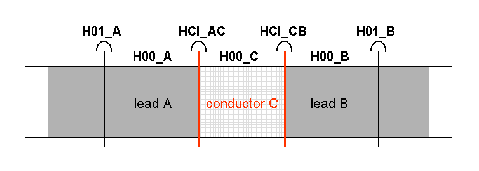
\includegraphics{acb.eps}\label{acb:ham}
\end{figure}
\begin{displaymath}
\begin{array}{lll}
\textrm{H00\_A} &=& \textrm{N}\times\textrm{N on site hamiltonian
of the leads A (H00 from bulk calculation)}\\
\textrm{H01\_A} &=& \textrm{N}\times\textrm{N hopping hamiltonian
of the leads A (H01 from bulk calculation)}\\
\textrm{H00\_B} &=& \textrm{P}\times\textrm{P on site hamiltonian
of the leads B (H00 from bulk calculation)}\\
\textrm{H01\_B} &=& \textrm{P}\times\textrm{P hopping hamiltonian
of the leads B (H01 from bulk calculation)}\\
\textrm{H00\_C} &=& \textrm{M}\times\textrm{M on site hamiltonian
of the conductor C (H00 from bulk calculation)}\\
\textrm{HCI\_AC} &=& \textrm{N}\times\textrm{M coupling matrices
between lead A and conductor C}\\
\textrm{HCI\_CB} &=& \textrm{M}\times\textrm{P coupling matrices
between conductor C and lead B}\\
\textrm{ } &\textrm{ }& \textrm{the coupling matrices have to be
adapted from H01 of supercell calculation}
\end{array}
\end{displaymath}

\noindent \underline{NOTES}: (i) The definition of the coupling
matrices HCI\_ {\bf MUST BE DONE CAREFULLY case by case},
depending on the particular system definition. (ii) In order to
match the hamiltonian matrices at the boundary, it is necessary to
check that the diagonal elements of the H00 matrices were aligned.
If not a rigid shift must be done.
